\documentclass{beamer}
%Information to be included in the title page:
% \title{Sample title}
% \author{Anonymous}
% \institute{Overleaf}
\usepackage{xcolor}
\usepackage{booktabs}
\usepackage{graphicx}
\usepackage{subcaption}
\usepackage[]{hyperref}

\usetheme[]{default}
\begin{document}
\renewcommand{\d}{\: \mathrm{d} }
\newcommand{\e}{\mathrm{e}}


\title[] {Recitation Class for Mid II \\ Chapter 6 - 9}

\author[lzx]{Zexi Li}

\institute[email]{lzx12138@sjtu.edu.cn}

\date{2021.07.06}

\frame{\titlepage}

\AtBeginSection[]
{
    \begin{frame}
        \frametitle{Table of Contents}
        \tableofcontents[currentsection]
    \end{frame}
}

\begin{frame}
    \frametitle{Outline}
    \tableofcontents
\end{frame}

\section{Overview}
    \begin{frame} \frametitle{Overview}
        \begin{itemize}
            \item \textbf{Chapter 9} Metal–Semiconductor and Semiconductor Heterojunctions
            \begin{figure}[H]
                \centering
                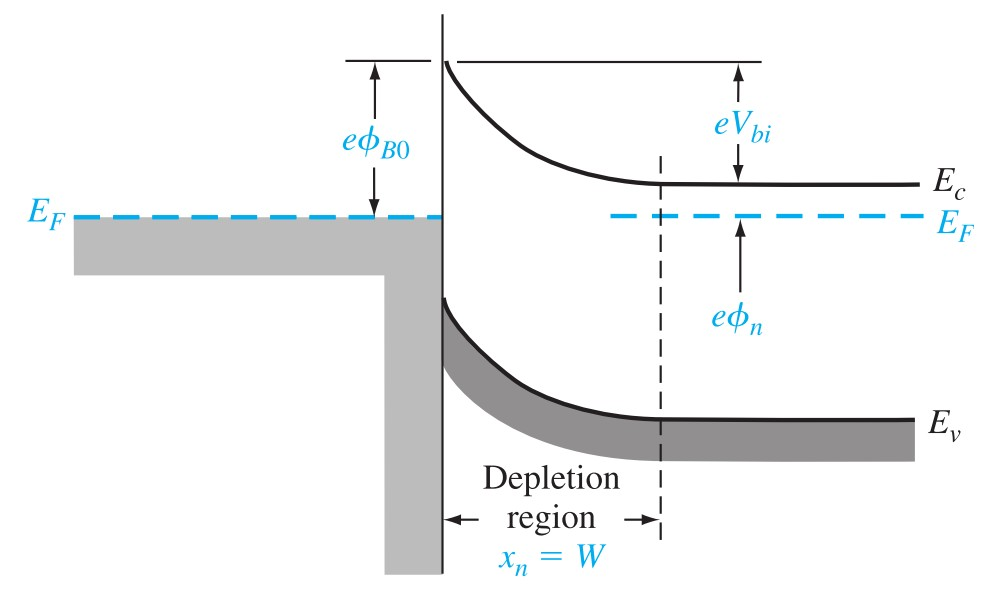
\includegraphics[width=0.6\linewidth]{C9-overview.jpg}
                \label{fig:C9-overview.jpg}
            \end{figure}
            \item \textbf{Chapter 7 \& 8} The pn Junction and pn Junction Diode
            \begin{minipage}{\linewidth}
                \centering
                \begin{minipage}{0.49\linewidth}
                    \begin{figure}[H]
                        \centering
                        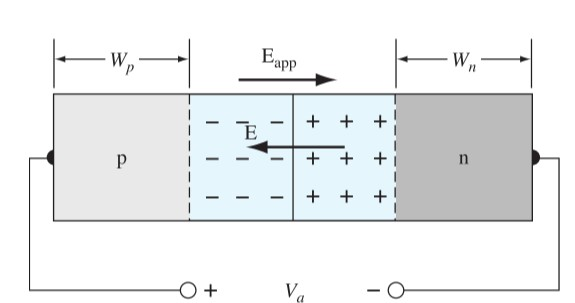
\includegraphics[width=\linewidth]{C8-overview-1.jpg}
                        \label{fig:C8-overview-1.jpg}
                    \end{figure}
                \end{minipage}
                \begin{minipage}{0.49\linewidth}
                    \begin{figure}[H]
                        \centering
                        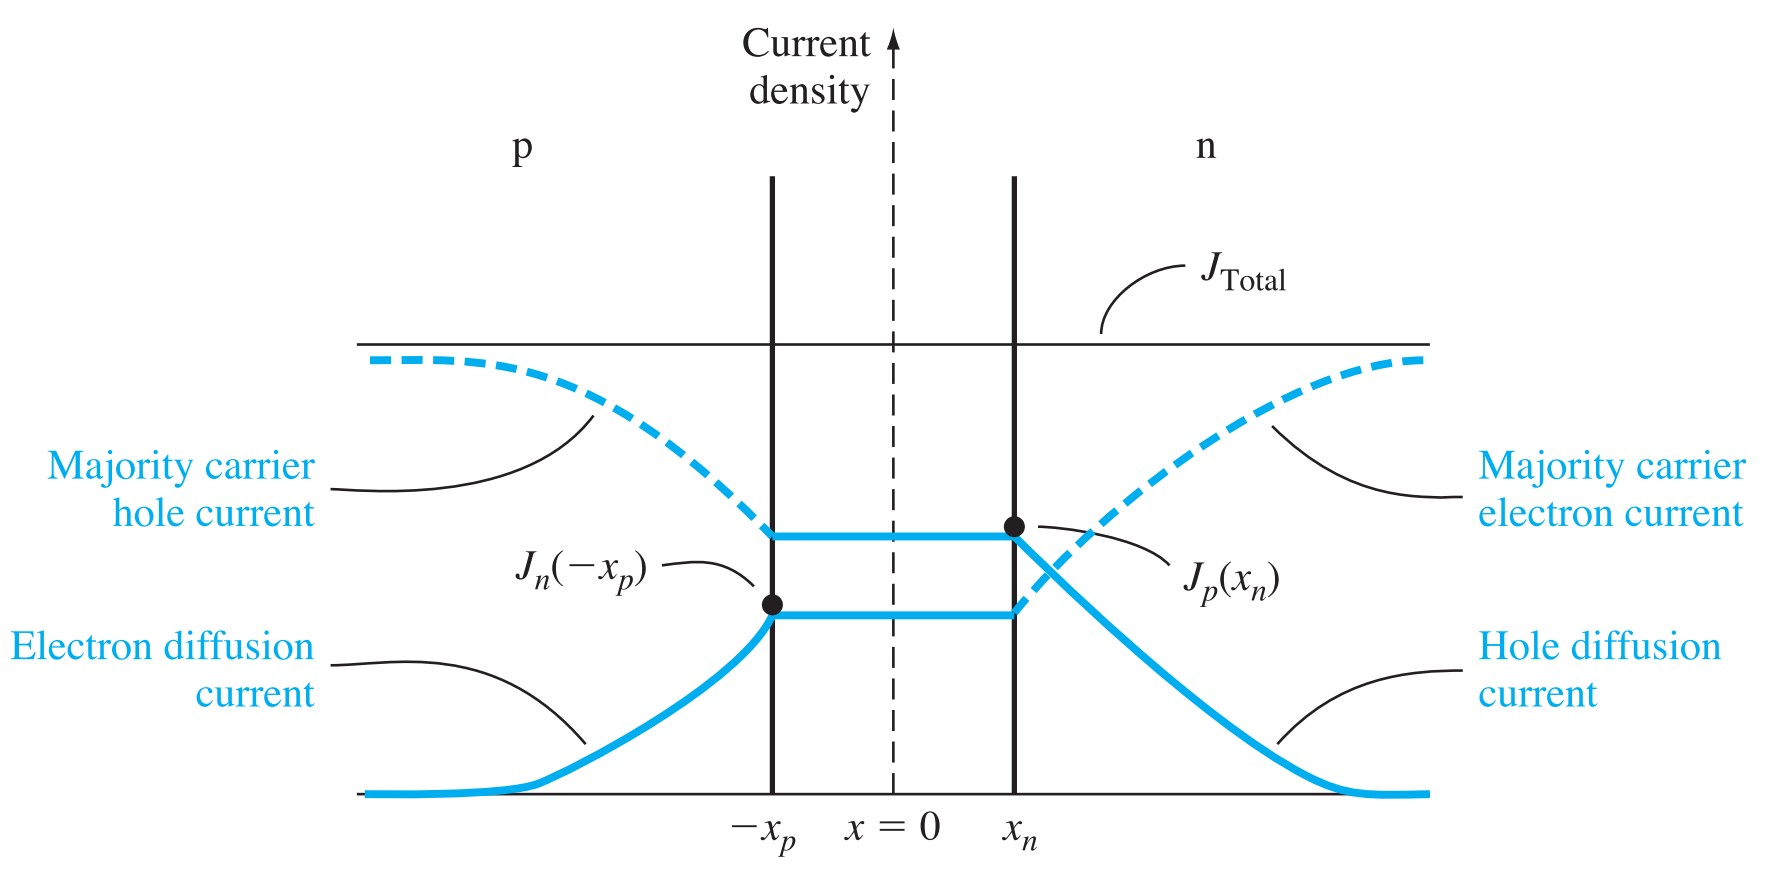
\includegraphics[width=\linewidth]{C8-overview-2.jpg}
                        \label{fig:C8-overview-2.jpg}
                    \end{figure}
                \end{minipage}
            \end{minipage}
        \end{itemize}
    \end{frame}
    \begin{frame} \frametitle{Overview}
        \begin{itemize}
            \item \textbf{Chapter 6} Nonequilibrium Excess Carriers in Semiconductors
                \begin{equation*}
                    \begin{aligned}
                        D_n \frac{\d^2 (\delta n)}{\d x^2} + \mu_n \left( E \frac{\d (\delta n)}{\d x} + n \frac{\d E}{\d x}  \right) + g_n - \frac{n}{\tau_{nt}} = \frac{\d (\delta n)}{\d t} \\
                        D_p \frac{\d^2 (\delta p)}{\d x^2} - \mu_p \left( E \frac{\d (\delta p)}{\d x} + p \frac{\d E}{\d x}  \right) + g_p - \frac{p}{\tau_{pt}} = \frac{\d (\delta p)}{\d t} \\
                    \end{aligned}
                \end{equation*}
        \end{itemize}
    \end{frame}

\section{Chapter 6 Nonequilibrium Excess Carriers in Semiconductors}
    \begin{frame} \frametitle{Electron-hole Generation \& Recombination}
        \begin{figure}[H]
            \centering
            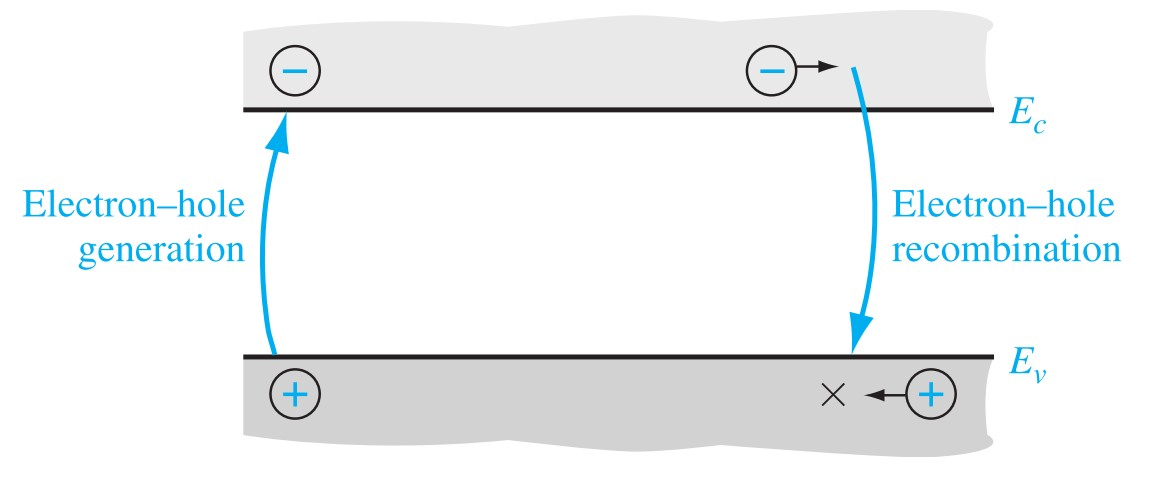
\includegraphics[width=0.6\linewidth]{Generation-recombination.jpg}
            \label{fig:Generation-recombination.jpg}
        \end{figure}
        \begin{equation*}
            G_{n0} = G_{p0}, \quad R_{n0} = R_{p0}
        \end{equation*}
    \end{frame}

    \begin{frame} \frametitle{Thermal-equilibrium}
        \textcolor{blue}{Thermal-equilibrium}: the net carrier concentrations are independent of time, which means that the generation and recombination of electrons and holes are equal.
        \begin{equation*}
            G_{n0} = G_{p0} = R_{n0} = R_{p0}
        \end{equation*}

        \textcolor{blue}{Nonequilibrium}: 
        
        \begin{minipage}{\linewidth}
            \begin{minipage}{0.5\linewidth}
                \begin{equation*}
                    \begin{aligned}
                        n &= n_0 + \delta n \\
                        p &= p_0 + \delta p
                    \end{aligned}
                \end{equation*}
                \par Note that $np \neq n_0 p_0 = n_i^2$.
            \end{minipage}
            \begin{minipage}{0.49\linewidth}
                \begin{figure}[H]
                    \centering
                    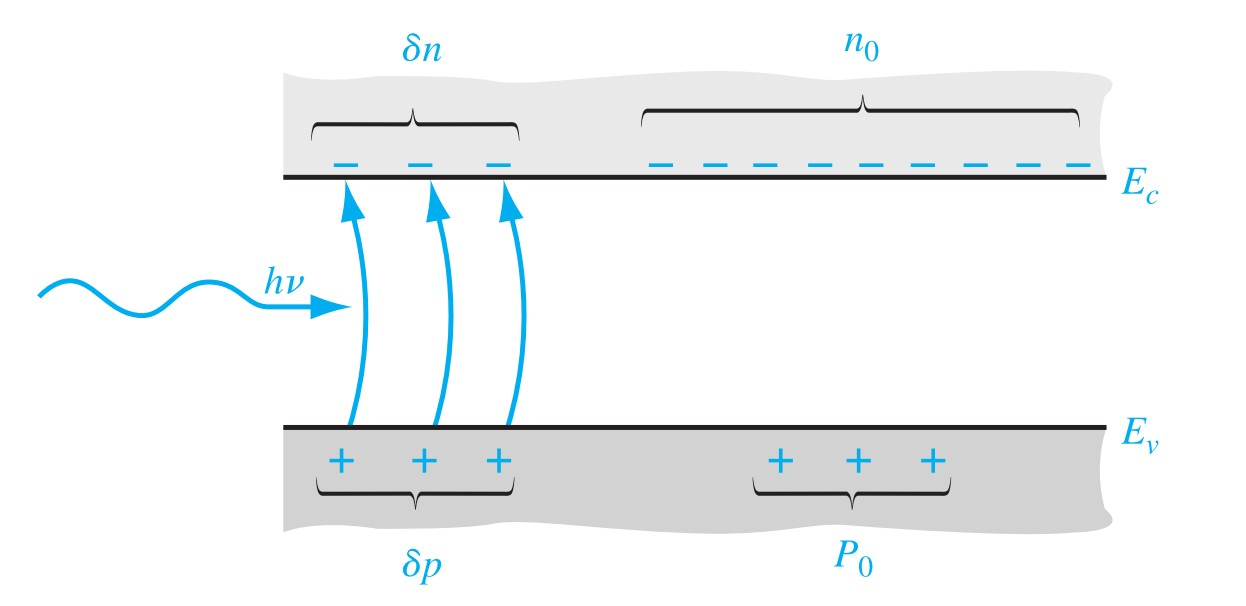
\includegraphics[width=\linewidth]{Photons-generation.jpg}
                    \caption{Creation of excess electron and hole densities by photons}
                    \label{fig:Photons-generation.jpg}
                \end{figure}
            \end{minipage}
        \end{minipage}
    \end{frame}

    \begin{frame} \frametitle{Net Recombination Rate}
        n-type:
        \begin{equation*}
            R^\prime_n = R^\prime_p = \frac{\delta p(t)}{\tau_{p0}}
        \end{equation*}
        p-type:
        \begin{equation*}
            R^\prime_n = R^\prime_p = \frac{\delta n(t)}{\tau_{n0}} 
        \end{equation*}
    \end{frame}

    \begin{frame} \frametitle{Quasi-Fermi Energy Level}
        \begin{equation*}
            \begin{aligned}
                n_0 + \delta n &= n_i \exp \left( \frac{E_{Fn} - E_{Fi}}{kT}  \right) \\
                p_0 + \delta p &= n_i \exp \left( \frac{E_{Fi} - E_{Fp}}{kT}  \right) \\
            \end{aligned}
        \end{equation*}
        \begin{figure}[H]
            \centering
            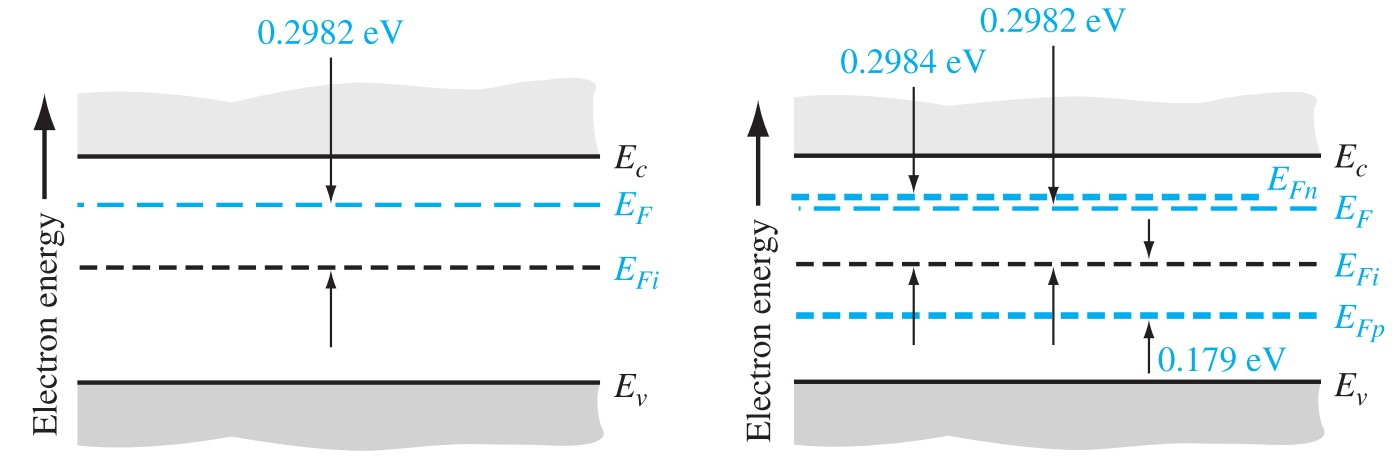
\includegraphics[width=\linewidth]{Quasi-fermi-level-C5.jpg}
            \label{fig:Quasi-fermi-level-C5.jpg}
        \end{figure}
    \end{frame}

    % \begin{frame} \frametitle{Question}
    %     \textcolor{blue}{Why we only consider minority excess carrier?} \\
    %     \par Consider the case where we have a n-type silicon semiconductor, with $n_0 = 10^{17}cm ^{-3}$, and $p_0 = n_i^2 / n_0 = 2250cm^{-3}$. And the excess carrier $\delta n = 10^{14} cm^{-3}$, which is only $0.1\%$ of $n_0$. However, $\delta p = \delta n = 10^{14} cm^{-3}$, which is greatly larger than $p_0$.
    %     \par You can also have such feeling from the Quasi-Fermi Energy Level diagram that $E_{Fn}$ is close to $E_F$ while $E_{Fp}$ changes a lot.
    % \end{frame}

    \begin{frame} \frametitle{Excess Carrier Lifetime}
        \begin{equation*}
            \boxed{
                \begin{aligned}
                    R_n = R_p &= \frac{C_n C_p N_t (np - n_i^2)}{C_n (n + n^\prime) + C_p(p + p^\prime)} \\
                    &= \frac{(np - n_i^2)}{\tau_{p0}(n + n^\prime) + \tau_{n0} (p + p^\prime) } 
                \end{aligned}
                }
        \end{equation*}
        where 
        \begin{equation*}
            \resizebox*{\textwidth}{!}{ %
                $n^\prime = N_c \exp\left[ - \dfrac{E_c - E_t}{kT}  \right], p^\prime = N_v \exp \left[ - \dfrac{E_t - E_v}{kT}  \right], \text{ and } \tau_{n0} = \dfrac{1}{C_n N_t}$
            }
        \end{equation*}
    \end{frame}

    \begin{frame} \frametitle{Surface Effects}
        \begin{figure}[H]
            \centering
            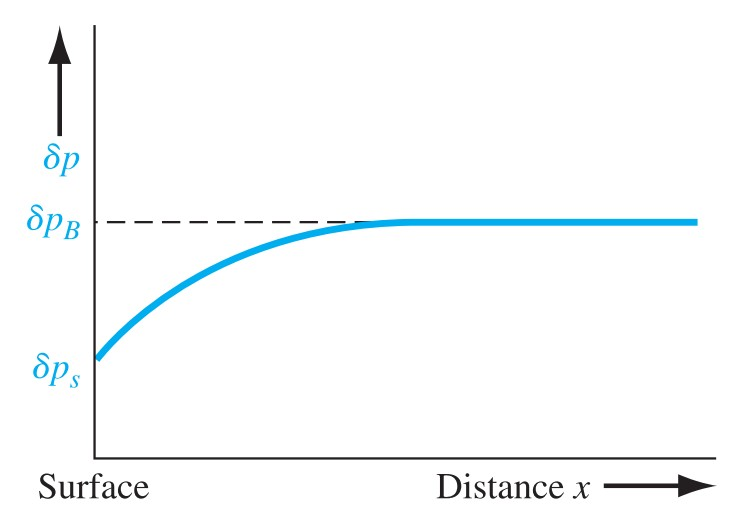
\includegraphics[width=0.6\linewidth]{Suerface-concentration.jpg}
            \label{fig:Suerface-concentration.jpg}
        \end{figure}
        \begin{equation*}
            \begin{aligned}
                \boxed{- D_p \left. \left[ \hat{n} \cdot \frac{\d (\delta p)}{\d x}  \right] \right|_{\text{surf}} = s \; \delta p |_{\text{surf}}}
            \end{aligned}
        \end{equation*}
        \begin{equation*}
            \begin{aligned}
                \delta p(x) = g^\prime \tau_{p0} \left( 1 - \frac{sL_p\e^{-x/L_p} }{D_p + sL_p}  \right)
            \end{aligned}
        \end{equation*}
    \end{frame}

    \begin{frame} \frametitle{Time-dependent Continuity Equation}
        \begin{equation*}
            \boxed{
                \begin{aligned}
                    D_n \frac{\d^2 n}{\d x^2} + \mu_n \left( E \frac{\d n}{\d x} + n \frac{\d E}{\d x}  \right) + g_n - \frac{n}{\tau_{nt}} = \frac{\d n}{\d t} \\
                    D_p \frac{\d^2 p}{\d x^2} - \mu_p \left( E \frac{\d p}{\d x} + p \frac{\d E}{\d x}  \right) + g_p - \frac{p}{\tau_{pt}} = \frac{\d p}{\d t} \\
                \end{aligned}
            }
        \end{equation*}
        \par For homogeneous semiconductor, $n(x) = n_0 + \delta n(x)$, the equation can be simplified to 
        \begin{equation*}
            \boxed{
                \begin{aligned}
                    D_n \frac{\d^2 (\delta n)}{\d x^2} + \mu_n \left( E \frac{\d (\delta n)}{\d x} + n \frac{\d E}{\d x}  \right) + g_n - \frac{n}{\tau_{nt}} = \frac{\d (\delta n)}{\d t} \\
                    D_p \frac{\d^2 (\delta p)}{\d x^2} - \mu_p \left( E \frac{\d (\delta p)}{\d x} + p \frac{\d E}{\d x}  \right) + g_p - \frac{p}{\tau_{pt}} = \frac{\d (\delta p)}{\d t} \\
                \end{aligned}
            }
        \end{equation*}
        \begin{equation*}
            \boxed{
                g_n - \frac{n}{\tau_{pt}} = g^\prime - \frac{\delta n}{\tau_{pt} }  
            }
        \end{equation*}
    \end{frame}

    \begin{frame} \frametitle{Equation Simplification}
        \begin{figure}[H]
            \centering
            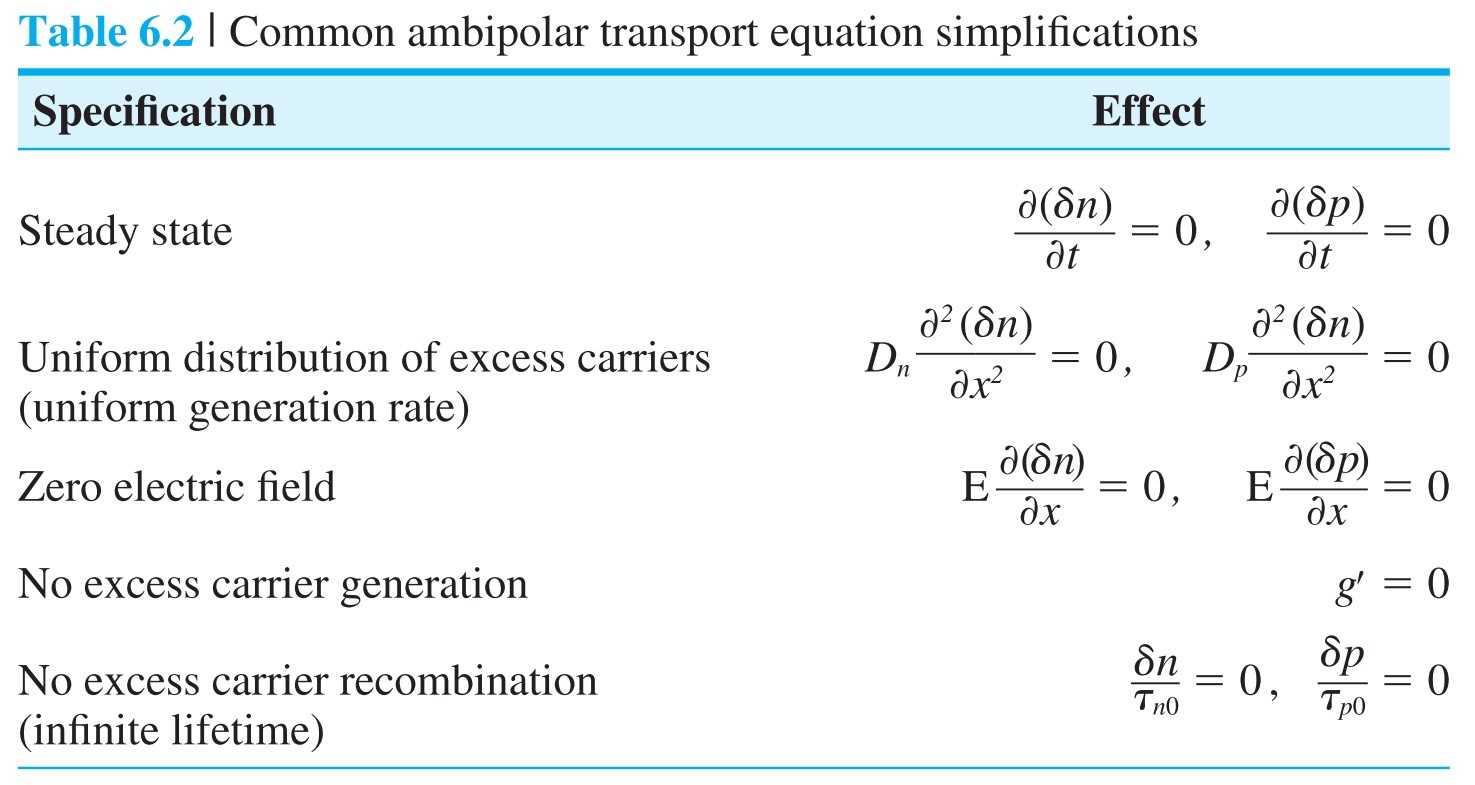
\includegraphics[width=0.9\linewidth]{Equation-simplification.jpg}
            \label{fig:Equation-simplification.jpg}
        \end{figure}
    \end{frame}

    \begin{frame} \frametitle{Equation General Solution}
        \par See cheating paper.
    \end{frame}

\section{Chapter 7 The pn junction}
    \begin{frame}[t] \frametitle{Built-in Potential Barrier}
        \begin{figure}[H]
            \centering
            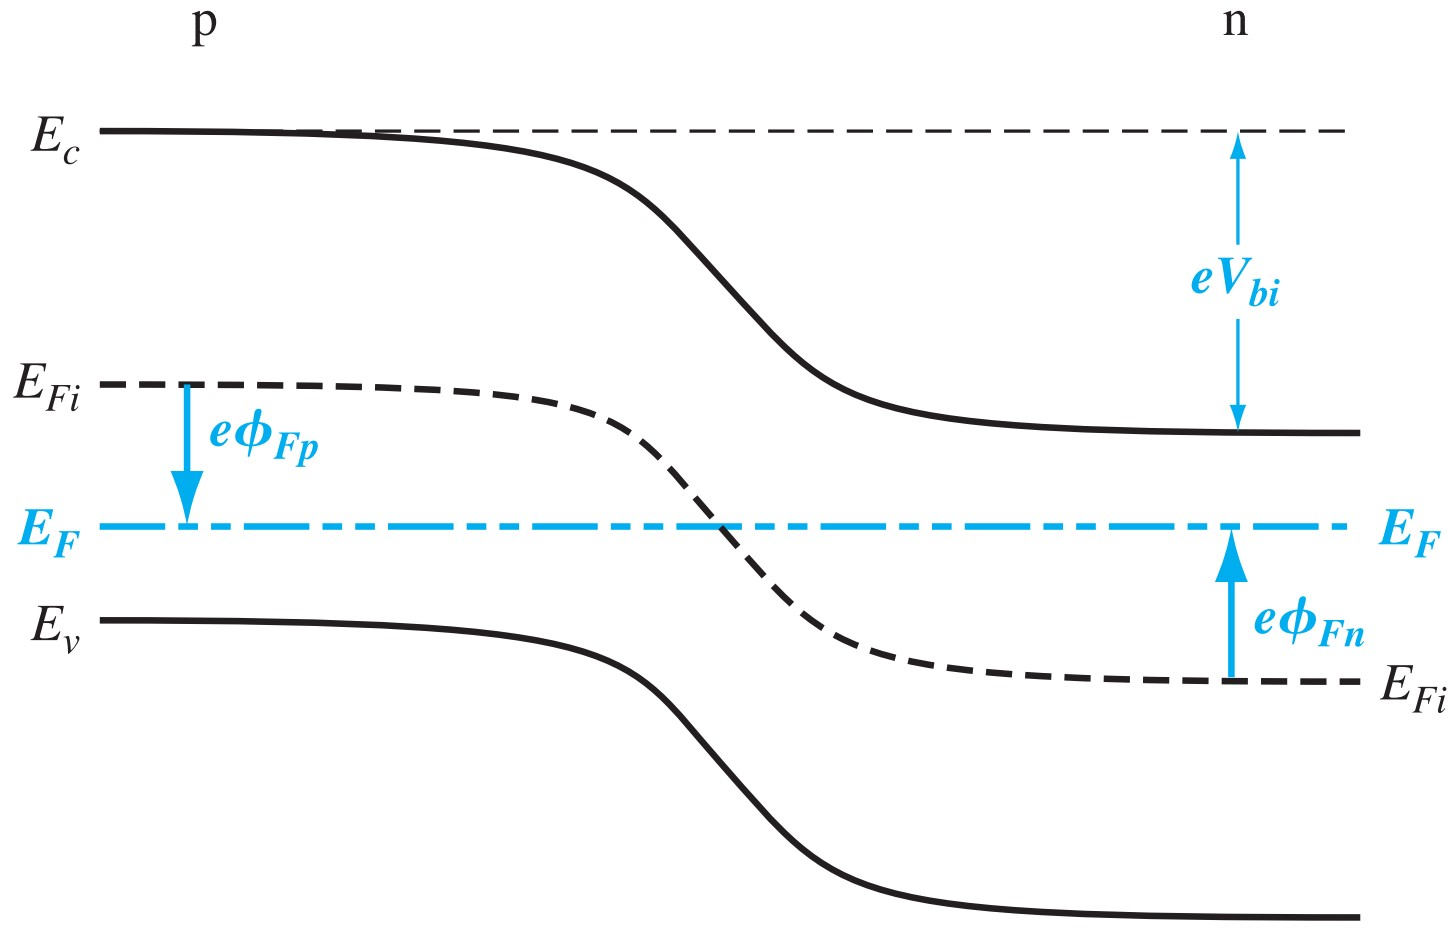
\includegraphics[width=0.5\linewidth]{pn-junction-energy-band-diagram.jpg}
            \label{fig:pn-junction-energy-band-diagram-2.jpg}
        \end{figure}
        \begin{equation*}
            % \color{pink}
            \boxed{
                \begin{aligned}
                    V_{bi} &= |\phi_{Fn}| + |\phi_{Fp}| \\
                    &= \frac{kT}{e} \ln \left( \frac{N_a N_d}{n_i^2}  \right) = V_t \ln\left( \frac{N_a N_d}{n_i^2}  \right)
                \end{aligned}
            }
        \end{equation*}
        \par $V_{bi}$: built-in potential barrier.
        \par $V_t = kT / e$ defined as the thermal voltage.
    \end{frame}

    \begin{frame} \frametitle{Zero Applied Bias}
        \begin{minipage}{\linewidth}
            \begin{minipage}[b]{0.49\linewidth}
                \begin{figure}[H]
                    \centering
                    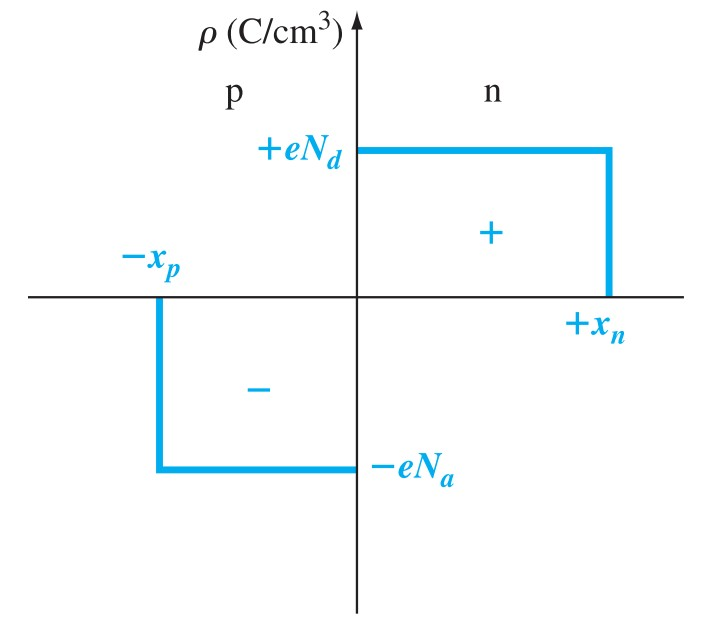
\includegraphics[width=0.95\linewidth]{Space-charge-density.jpg}
                    \caption{space charge density}
                    \label{fig:Space-charge-density.jpg}
                \end{figure}
                \begin{equation*}
                    N_a x_p = N_d x_n
                \end{equation*}
            \end{minipage}
            \begin{minipage}[b]{0.49\linewidth}
                \begin{figure}[H]
                    \centering
                    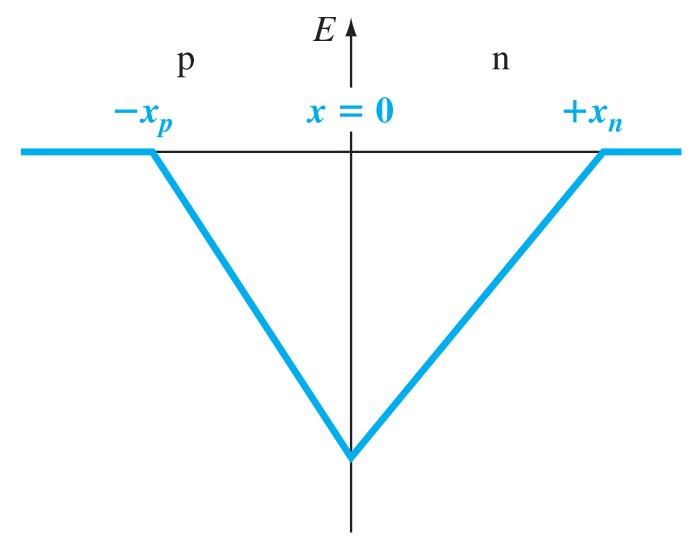
\includegraphics[width=0.95\linewidth]{pn-junction-electric-field.jpg}
                    \caption{electric field}
                    \label{fig:pn-junction-electric-field.jpg}
                \end{figure}
                \begin{equation*}
                    |k| = \frac{e N_{a/d}}{\varepsilon_s} 
                \end{equation*}
            \end{minipage}
        \end{minipage}
    \end{frame}

    \begin{frame} \frametitle{Zero Applied Bias}
        \fbox{
        \begin{minipage}{0.95\linewidth}
            \begin{equation*}
                N_a x_p = N_d x_n
            \end{equation*}
            \begin{equation*}
                \begin{aligned}
                    x_n &= \sqrt{\frac{2 \varepsilon_s \left( V_{bi} + V_R \right)}{e} \left[ \frac{N_a}{N_d}  \right]\left[ \frac{1}{N_a + N_d}  \right]} \\
                    x_p &= \sqrt{\frac{2 \varepsilon_s \left( V_{bi} + V_R \right)}{e} \left[ \frac{N_d}{N_a}  \right]\left[ \frac{1}{N_a + N_d}  \right]}
                \end{aligned}
            \end{equation*}
            \par $\varepsilon_s = \varepsilon_r \varepsilon_0$, where $\varepsilon_0 = 8.85 \times 10^{-14} F \cdot cm^{-1}$.
            \par $\varepsilon_r = 11.7$ for $Si$.

            \begin{equation*}
                W = x_n + x_p = \sqrt{\frac{2 \varepsilon_s \left( V_{bi} + V_R \right)}{e}  \left[ \frac{N_a + N_d}{N_a N_d}  \right]}
            \end{equation*}
        \end{minipage}
        }
    \end{frame}
    \begin{frame} \frametitle{Zero Applied Bias}
        \fbox{
        \begin{minipage}{0.95\linewidth}
            \begin{equation*}
                E = \left\{
                    \begin{aligned}
                        - \frac{eN_a}{\varepsilon_s} (x + x_p),\quad & - x_p \le x \le 0 \\
                        \frac{eN_d}{\varepsilon_s} (x_n - x),\quad & 0 \le x \le x_n  
                    \end{aligned}
                \right.
            \end{equation*}
            \begin{equation*}
                \begin{aligned}
                    |E_{max}| &= - \frac{eN_d x_n}{\varepsilon_s} = - \frac{e N_a x_p}{\varepsilon_s} \\ 
                    &= - \frac{2 (V_{bi} + V_R)}{W} 
                \end{aligned}
            \end{equation*}
            \begin{equation*}
                \phi(x) = - \int E(x) \d x
            \end{equation*}
        \end{minipage}
        }
    \end{frame}

    \begin{frame} \frametitle{Reverse Applied Bias}
        \begin{figure}[H]
            \centering
            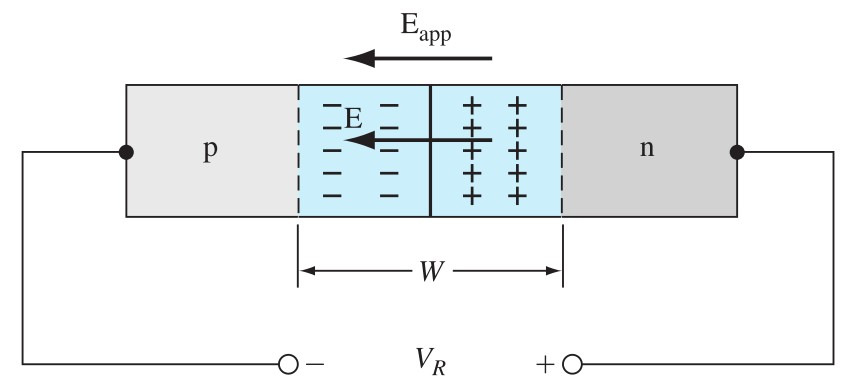
\includegraphics[width=0.5\linewidth]{Reversed-biase-graph.jpg}
            \label{fig:Reversed-biase-graph.jpg}
        \end{figure}
        \begin{figure}[H]
            \centering
            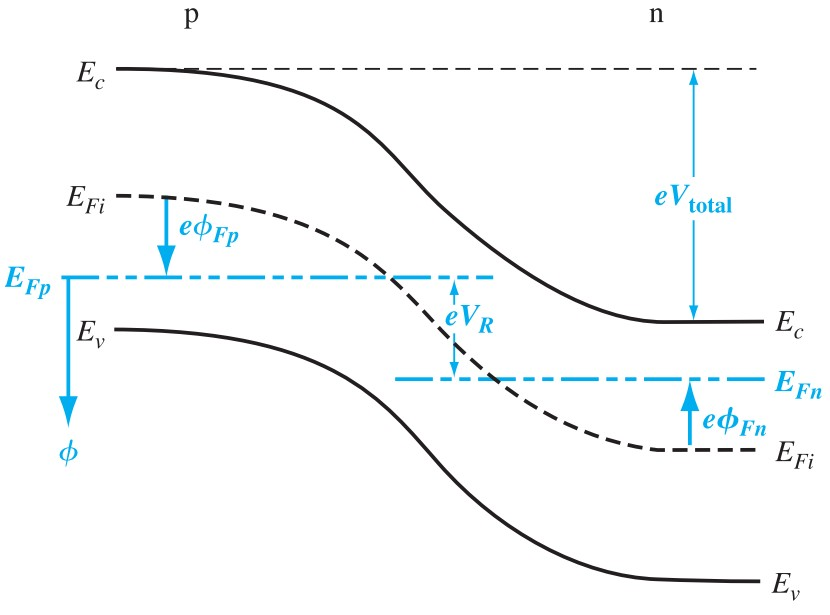
\includegraphics[width=0.5\linewidth]{Energy-band-diagram-reversed-biase.jpg}
            \caption{Energy-band diagram}
            \label{fig:Energy-band-diagram-reversed-biase.jpg}
        \end{figure}
    \end{frame}

    \begin{frame} \frametitle{Junction Capacitance}
        \begin{figure}[H]
            \centering
            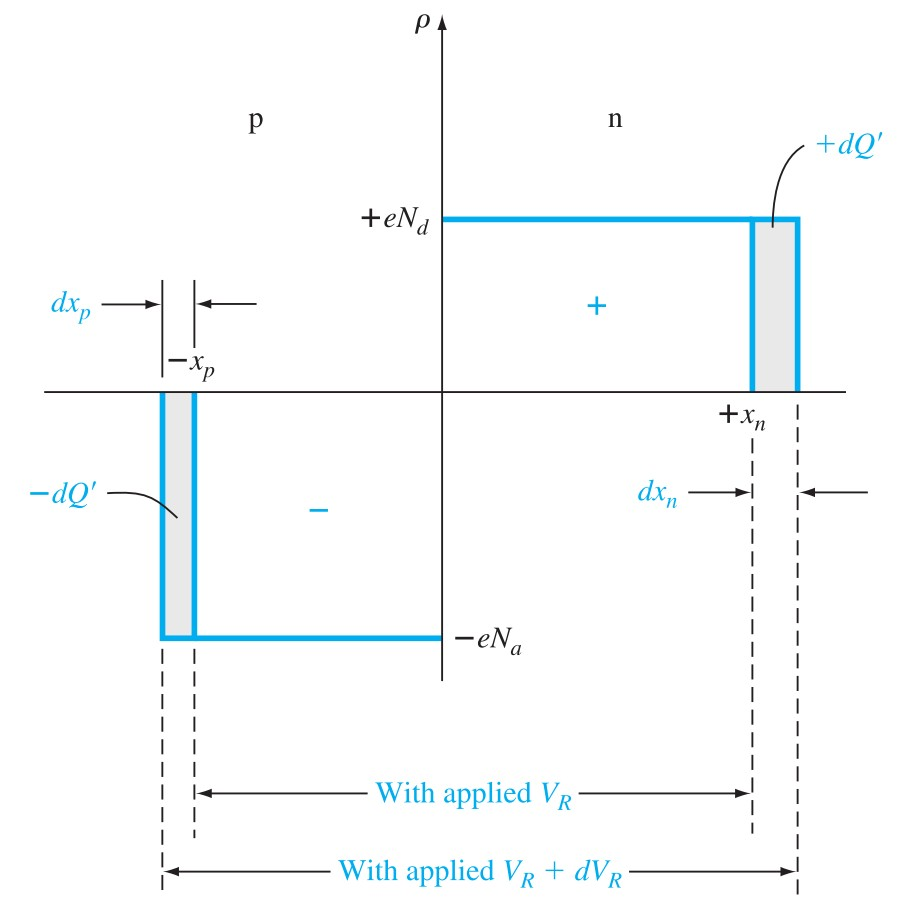
\includegraphics[width=0.6\linewidth]{Junction-capacitance.jpg}
            \caption{Differential change in the space charge width with a differential change in reverse-biased voltage for a uniformly doped pn junction}
            \label{fig:Junction-capacitance.jpg}
        \end{figure}
    \end{frame}

    \begin{frame} \frametitle{Junction Capacitance}
        \begin{equation*}
            \begin{aligned}
                C^\prime &= \frac{\d Q^\prime}{d V_R} \\
                d Q^\prime &= e N_d \d x_n = e N_a \d x_p
            \end{aligned}
        \end{equation*}
        \textcolor{orange}{$\d Q^\prime$ has units of $C/cm^2$, and $C^\prime$ has units of $F/cm^2$}.
        \begin{equation*}
            \boxed{C^\prime = \sqrt{\frac{e \varepsilon_s N_a N_d}{2 (V_{bi} + V_R) (N_a + N_d)} } = \frac{\varepsilon_s}{W} }
        \end{equation*}
    \end{frame}

    \begin{frame} \frametitle{One-sided Junciton}
        \begin{minipage}{\linewidth}
            \begin{minipage}{0.5\linewidth}
                \begin{equation*}
                    \begin{aligned}
                        & C^\prime \approx \sqrt{\frac{e \varepsilon_s N_d}{2 (V_{bi} + V_R)} } \\
                        \Rightarrow & \boxed{\left( \frac{1}{C^\prime}  \right)^2 = \frac{2(V_{bi} + V_R)}{e \varepsilon_s N_d} }
                    \end{aligned}
                \end{equation*}
                Experimentally determine $V_{bi}$ and $N_d$.
            \end{minipage}
            \hspace{2em}
            \begin{minipage}{0.4\linewidth}
                \begin{figure}[H]
                    \centering
                    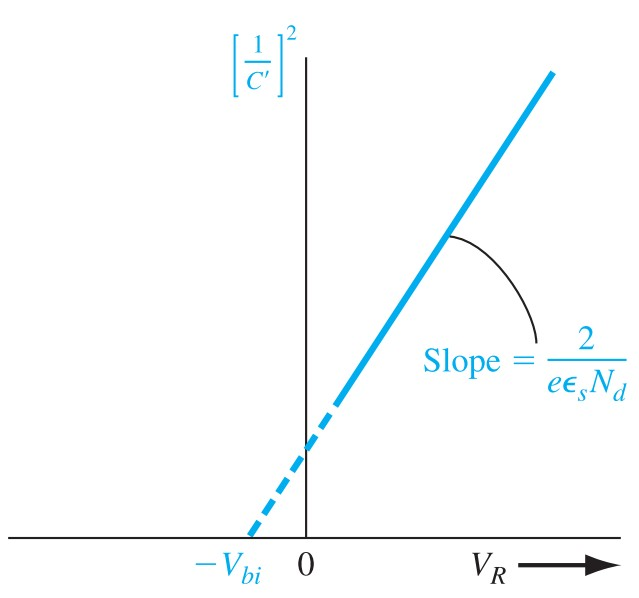
\includegraphics[width=\linewidth]{C-versus-VR.jpg}
                    \caption{$(1/C^\prime)^2$ versus $V_R$ of a \textcolor{orange}{uniformly} doped pn junction}
                    \label{fig:C-versus-VR.jpg}
                \end{figure}
            \end{minipage}
        \end{minipage}
    \end{frame}

\section{Chapter 8 The pn Junction Diode}
    \begin{frame} \frametitle{Charge Flow}
        \begin{figure}[H]
            \centering
            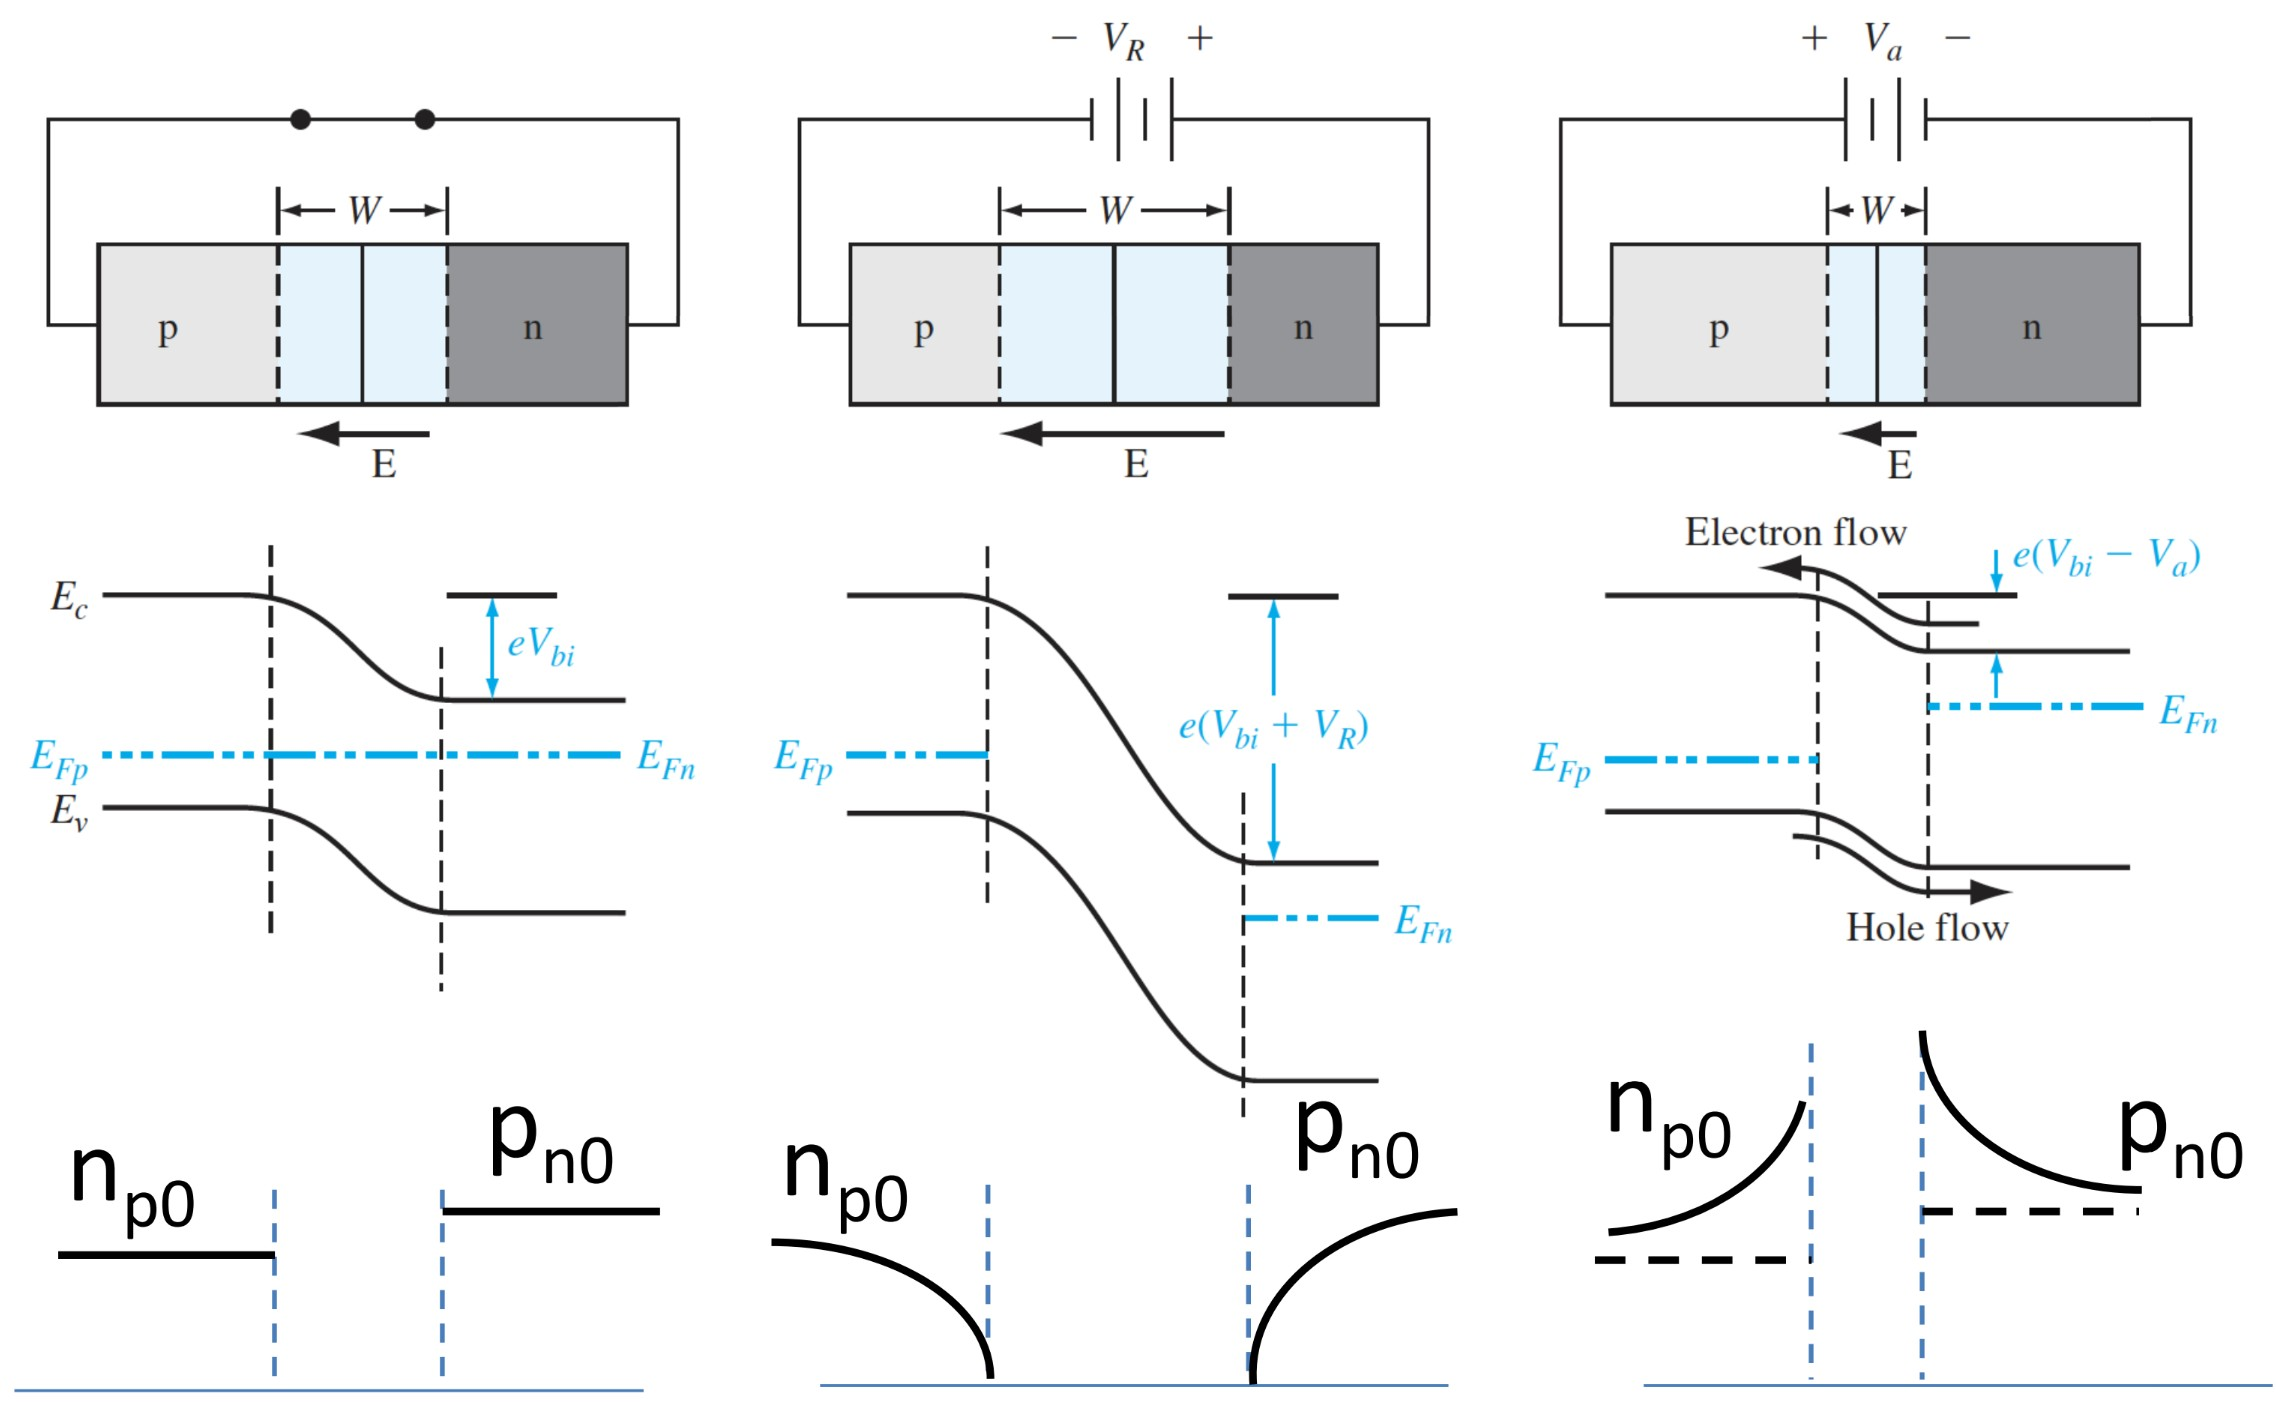
\includegraphics[width=\linewidth]{Charge-flow-in-pn-junction.jpg}
            \label{fig:Charge-flow-in-pn-junction.jpg}
        \end{figure}
    \end{frame}
    \begin{frame} \frametitle{Relation of Concentrations}
        \begin{equation*}
            \begin{aligned}
                n_{p0} = n_{n0} \exp\left( -\frac{e V_{bi} }{kT}  \right)
            \end{aligned}
        \end{equation*}
        \par Relates the minority carrier electron concentration on the p side of the junction to the majority carrier electron concentration on the n side of the junction in thermal equilibrium.
        \begin{equation*}
            \begin{aligned}
                V_{bi} &= V_t \ln \left( \frac{N_a N_d}{n_i^2}  \right)\\
                n_{n0} & \approx N_d \\
                n_{p0} & \approx \frac{n_i^2}{N_a}  \\
            \end{aligned}
        \end{equation*}
    \end{frame}

    \begin{frame} \frametitle{Forward Biased}
        \begin{figure}[H]
            \centering
            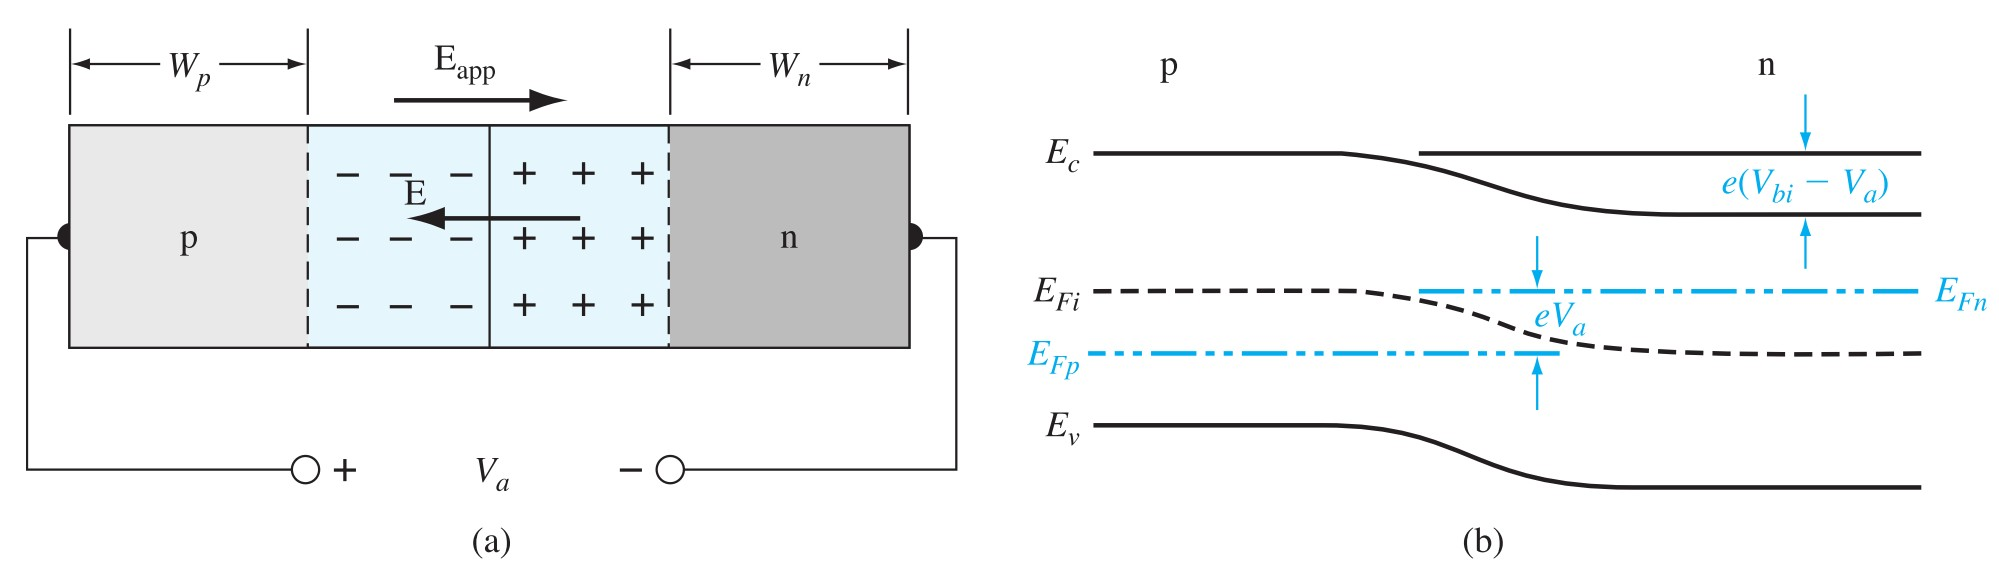
\includegraphics[width=0.9\linewidth]{Forward-biased-equation.jpg}
            \label{fig:Forward-biased-equation.jpg}
        \end{figure}
        \begin{equation*}
            \begin{aligned}
                n_p &= n_{n0} \exp\left( -\frac{e (V_{bi} - V_a)}{kT}  \right) \\
                &= n_{p0} \exp\left( \frac{eV_a}{kT}  \right)
            \end{aligned}
        \end{equation*}
    \end{frame}
    \begin{frame} \frametitle{Forward Biased}
        \begin{figure}[H]
            \centering
            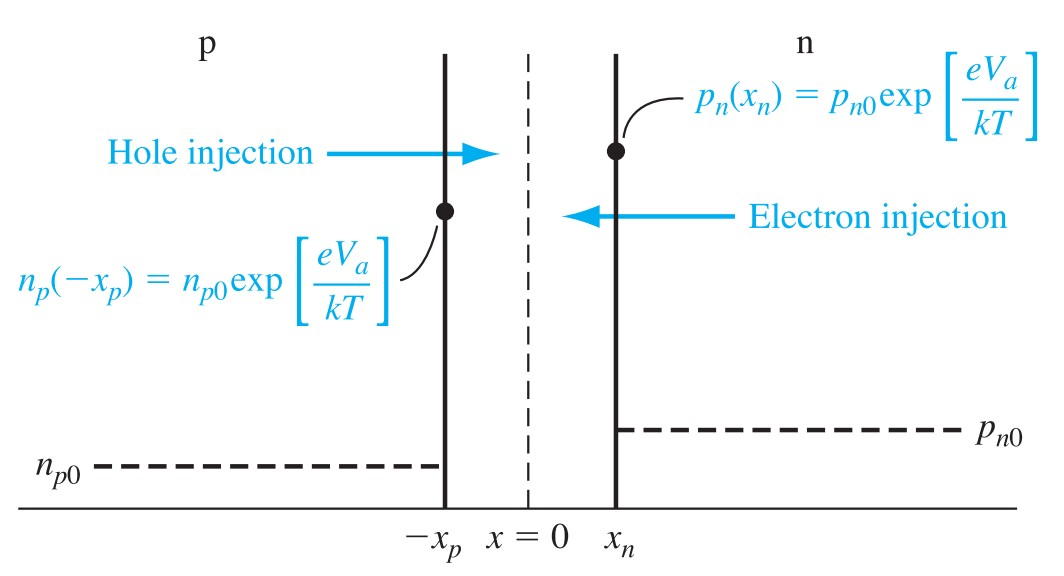
\includegraphics[width=0.8\linewidth]{Forward-biased-edge-concentration.jpg}
            \label{fig:Forward-biased-edge-concentration.jpg}
        \end{figure}
    \end{frame}

    \begin{frame} \frametitle{Minority Carrier Distribution}
        The solution is
        \begin{equation*}
            \resizebox*{\textwidth}{!}{
                \boxed{\delta p_n(x) = p_n(x) - p_{n0} = p_{n0} \left[ \exp\left( \dfrac{eV_a}{kT} \right) - 1\right] \exp\left( \dfrac{x_n - x}{L_p}  \right), \quad x \ge x_n}
            }
        \end{equation*}
        Similarly,
        \begin{equation*}
            \resizebox*{\textwidth}{!}{
                \boxed{\delta n_p(x) = n_p(x) - n_{p0} = n_{p0} \left[ \exp\left( \dfrac{eV_a}{kT}  \right) - 1 \right] \exp \left( \dfrac{x_p + x}{L_n}  \right), \quad x \le - x_p}
            }
        \end{equation*}
        \begin{figure}[H]
            \centering
            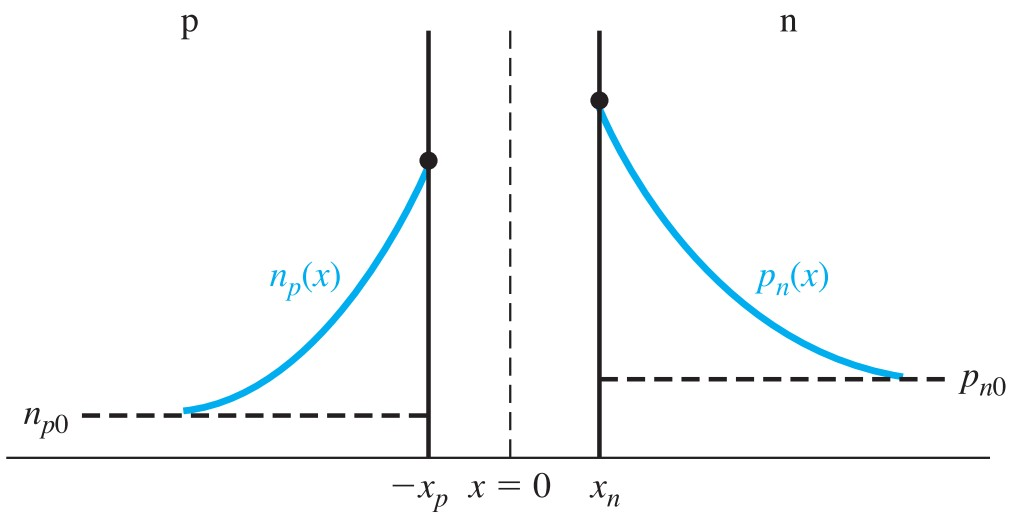
\includegraphics[width=0.6\linewidth]{Forward-biased-solution.jpg}
            \label{fig:Forward-biased-solution.jpg}
        \end{figure}
    \end{frame}

    \begin{frame} \frametitle{Quasi-Fermi Level}
        \begin{figure}[H]
            \centering
            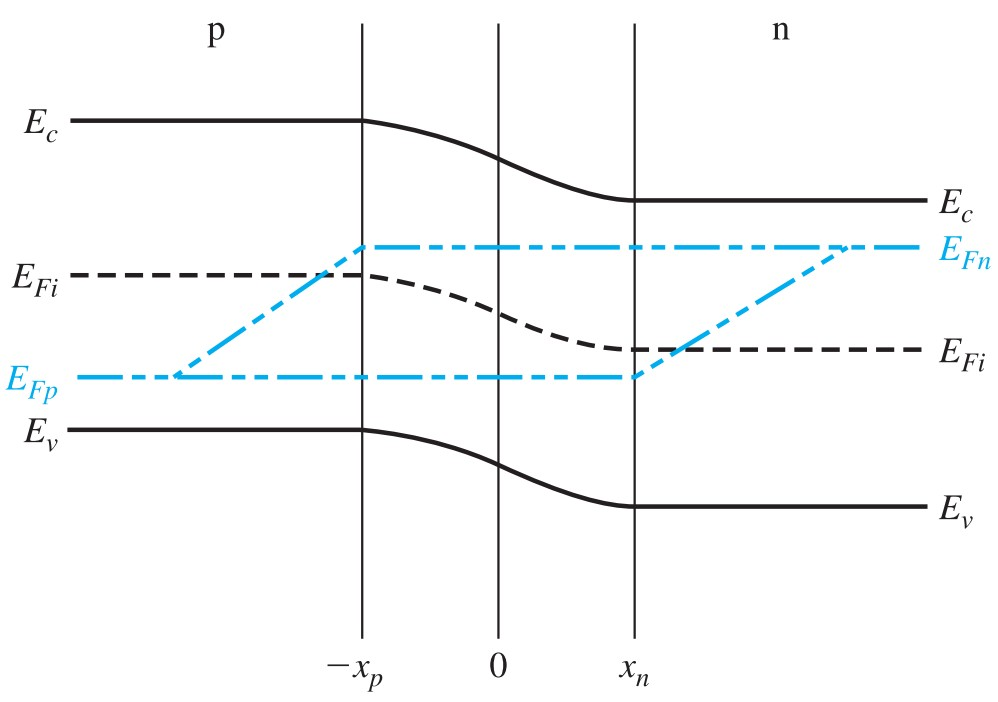
\includegraphics[width=0.5\linewidth]{Quasi-fermi-level.jpg}
            % \caption{Quasi-Fermi levels through a forward-biased pn junction.}
            \label{fig:Quasi-fermi-level-1.jpg}
        \end{figure}
        % \vspace{-2em}
        % \par In Chapter 6 there are equations
        \begin{equation*}
            p = p_0 + \delta p = n_i \exp\left( \frac{E_{Fi} - E_{Fp} }{kT}  \right)
        \end{equation*}
        \par Therefore the quasi-Fermi levels are linear functions of distance in the neutral p and n regions as shown in the Figure.
        \begin{equation*}
            np = n_i^2 \exp \left( \frac{E_{Fn} - E_{Fp} }{kT}  \right)
        \end{equation*}
    \end{frame}

    \begin{frame} \frametitle{Ideal - pn Junction Current}
        \begin{figure}[H]
            \centering
            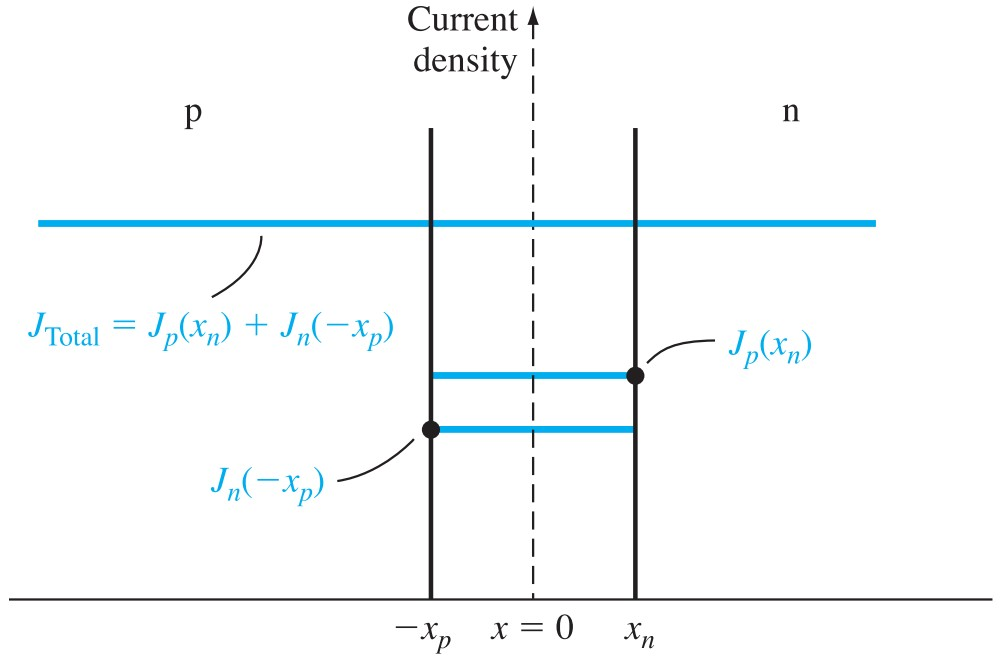
\includegraphics[width=0.6\linewidth]{Current-density.jpg}
            \label{fig:Current-density.jpg}
        \end{figure}
        \begin{equation*}
            J_p(x_n) = - e D_p \left. \frac{\d \left( \delta p_n(x) \right)}{\d x} \right|_{x = x_n}
        \end{equation*}
    \end{frame}
    \begin{frame} \frametitle{Ideal - pn Junction Current - Continue}
        \begin{equation*}
            \begin{aligned}
                J_{p} (x_n) &= \frac{e D_p p_{n0}}{L_p} \left[ \exp\left( \frac{eV_a}{kT}  \right) - 1 \right] \\
                J_{n} (-x_p) &= \frac{eD_n n_{p0} }{L_n} \left[ \exp\left( \frac{eV_a}{kT}  \right) - 1 \right]
            \end{aligned}
        \end{equation*}
        \par Then the total current density
        \begin{equation*}
            \boxed{
                \begin{aligned}
                    J &= J_s \left[ \exp\left( \frac{eV_a}{kT}  \right) - 1 \right] \\
                    & \qquad  \text{where } J_s = \left[ \frac{eD_p p_{n0} }{L_p} + \frac{eD_n n_{p0} }{L_n}  \right]
                \end{aligned}
            }
        \end{equation*}
    \end{frame}

    \begin{frame} \frametitle{Non-Ideal I - Generation-recombination currents}
        \begin{equation*}
            \begin{aligned}
                R_n &= \frac{(np - n_i^2)}{\tau_p \left[ n + n_i \exp \left( \frac{E_t - E_i}{kT}  \right) \right] + \tau_n \left[ p + n_i \exp \left( \frac{E_i - E_t}{kT}  \right) \right]} \\
                &= -\frac{n_i}{2\tau} = -G_0 \qquad \text{assume } E_t = E_i, \tau_n = \tau_p = \tau
            \end{aligned}
        \end{equation*}
        \begin{equation*}
            \begin{aligned}
                J_r &= \int_0^W q G_0 \d x \\
                &= \frac{qWn_i}{2\tau} 
            \end{aligned}
        \end{equation*}
        \begin{equation*}
            \begin{aligned}
                % J_{gen} &= \frac{en_i W}{2\tau_0} \\
                % J_{rec} &= J_{r0} \exp \left( \frac{eV_a}{2kT}  \right), \text{ where } J_{r0} = \frac{eWn_i}{2 \tau_0}  \\
                J = J_s \left[ \exp\left( \frac{qV_a}{kT}  \right)  - 1 \right] + \frac{q W n_i}{2\tau} \left[ \exp \left( \frac{qV_a}{2kT}  \right) - 1 \right]
            \end{aligned}
        \end{equation*}
    \end{frame}

    \begin{frame} \frametitle{Non-Ideal II - High Level Injection}
        \begin{figure}[H]
            \centering
            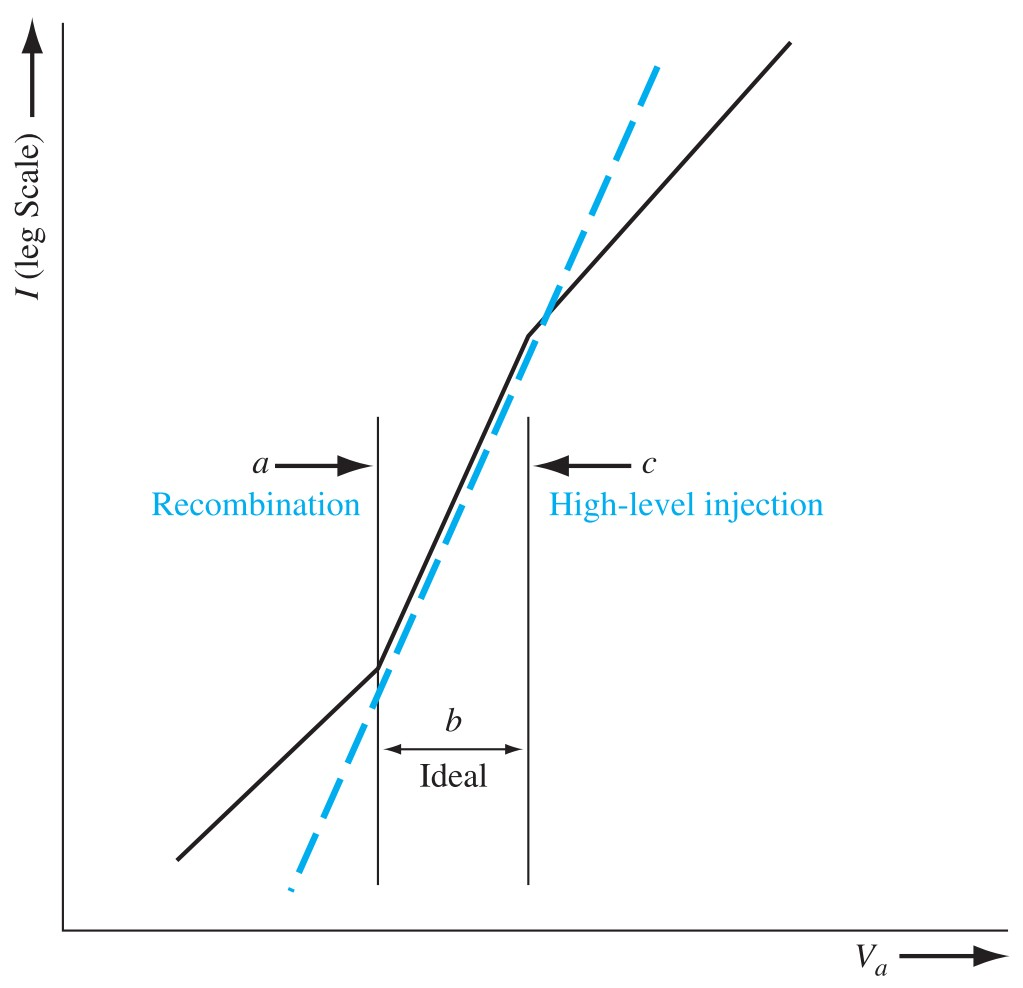
\includegraphics[width=0.6\linewidth]{High-level-injection.jpg}
            \label{fig:High-level-injection.jpg}
        \end{figure}
    \end{frame}

\section{Chapter 9 Metal–Semiconductor and Semiconductor Heterojunctions}

    \begin{frame} \frametitle{The Schottky Barrier Diode}
        \begin{minipage}{\linewidth}
            \begin{minipage}{0.45\linewidth}
                \begin{figure}[H]
                    \centering
                    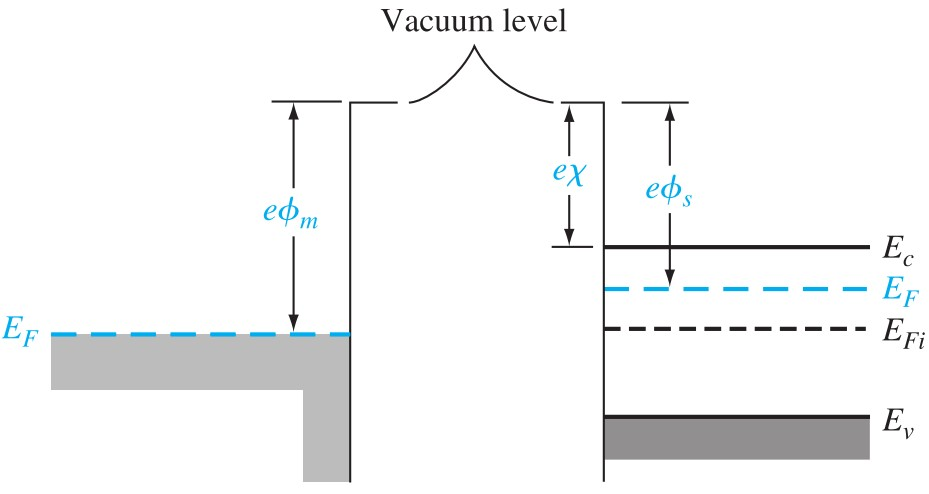
\includegraphics[width=\linewidth]{Work-function-graph.jpg}
                    \label{fig:Work-function-graph.jpg}
                \end{figure}
            \end{minipage}
            \begin{minipage}{0.45\linewidth}
                \begin{figure}[H]
                    \centering
                    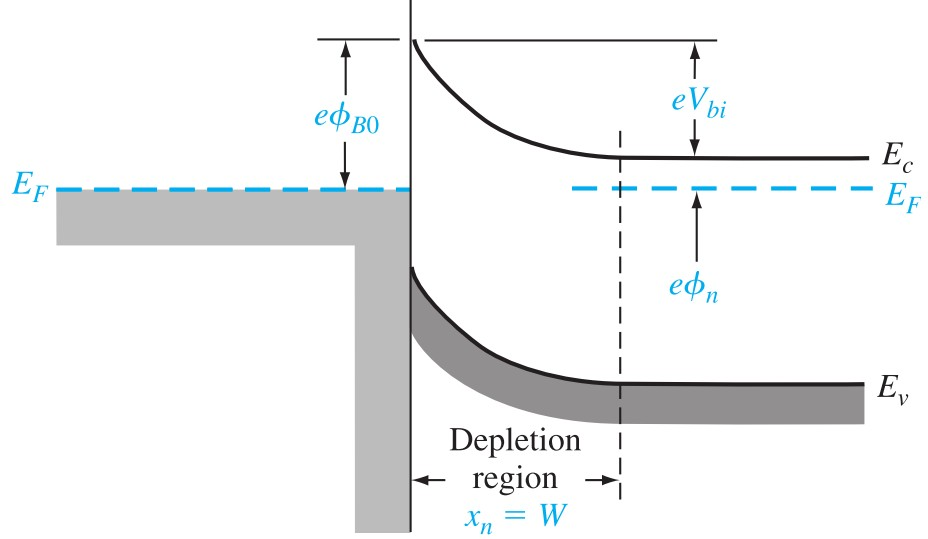
\includegraphics[width=\linewidth]{Ideal-energy-band-diagram-after-contact.jpg}
                    \label{fig:Ideal-energy-band-diagram-after-contact.jpg}
                \end{figure}
            \end{minipage}
        \end{minipage}
        \par Work function: $\phi$
        \par Electron affinity: $\chi$
        \par Schottky barrier: $\phi_{B0} = \phi_m - \chi$
        \par Built-in potential barrier: $V_{bi} = \phi_{B0} - \phi _n$
    \end{frame}

    \begin{frame} \frametitle{Non-ideal Effects - Schottky Barrier Lowering}
        \begin{figure}[H]
            \centering
            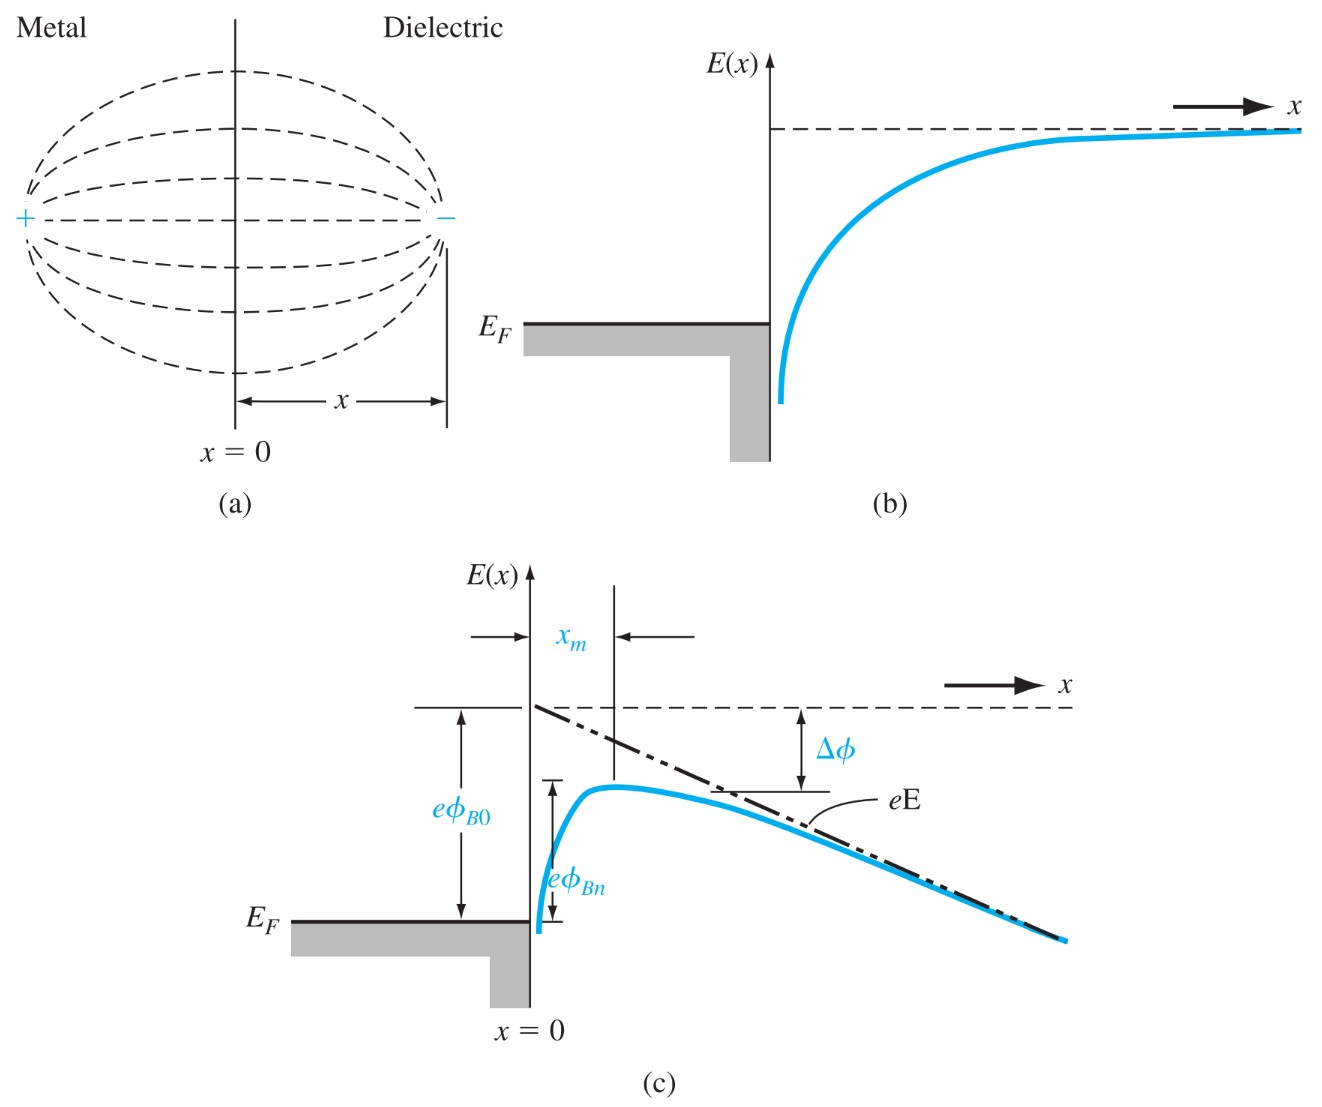
\includegraphics[width=0.9\linewidth]{Schottky-barrier-lowering.jpg}
            \label{fig:Schottky-barrier-lowering.jpg}
        \end{figure}
    \end{frame}
    \begin{frame} \frametitle{Non-ideal Effects - Schottky Barrier Lowering}
        \begin{equation*}
            \begin{aligned}
                &F = \frac{-e^2}{4 \pi \varepsilon_s (2x)^2} = -eE \\
                &-\phi(x) = + \int_x^\infty E \d x^\prime = \frac{-e}{16\pi \varepsilon_s x} \\ 
                \text{With electric field: } & -\phi(x) = \frac{-e}{16 \pi \varepsilon_s x} - Ex  \\
                \frac{\d (e \phi(x))}{\d x} = 0 \quad \Rightarrow \quad & \Delta \phi = \sqrt{\frac{eE}{4\pi \varepsilon_s} }  
            \end{aligned}
        \end{equation*}
    \end{frame}

    \begin{frame} \frametitle{Current-Voltage Relationship}
        \begin{equation*}
            \begin{aligned}
                J &= J_{sT} \left[ \exp\left( \frac{eV_a}{kT}  \right) - 1 \right] \\
                J_{sT} &= A^* T^2 \exp \left( \frac{-e \phi_{Bn} }{kT}  \right) \\
                A^* &= \frac{4\pi e m_n^* k^2}{h^3} 
            \end{aligned}
        \end{equation*}
        \par $A^*$: effective Richardson constant for thermionic emission.
        \par \textcolor{orange}{(After plugging in all values, times $10^{-4}$ to get the unit $A \cdot K^{-2} \cdot cm^{-2}$)}
    \end{frame}

    \begin{frame} \frametitle{}
        \begin{figure}[H]
            \centering
            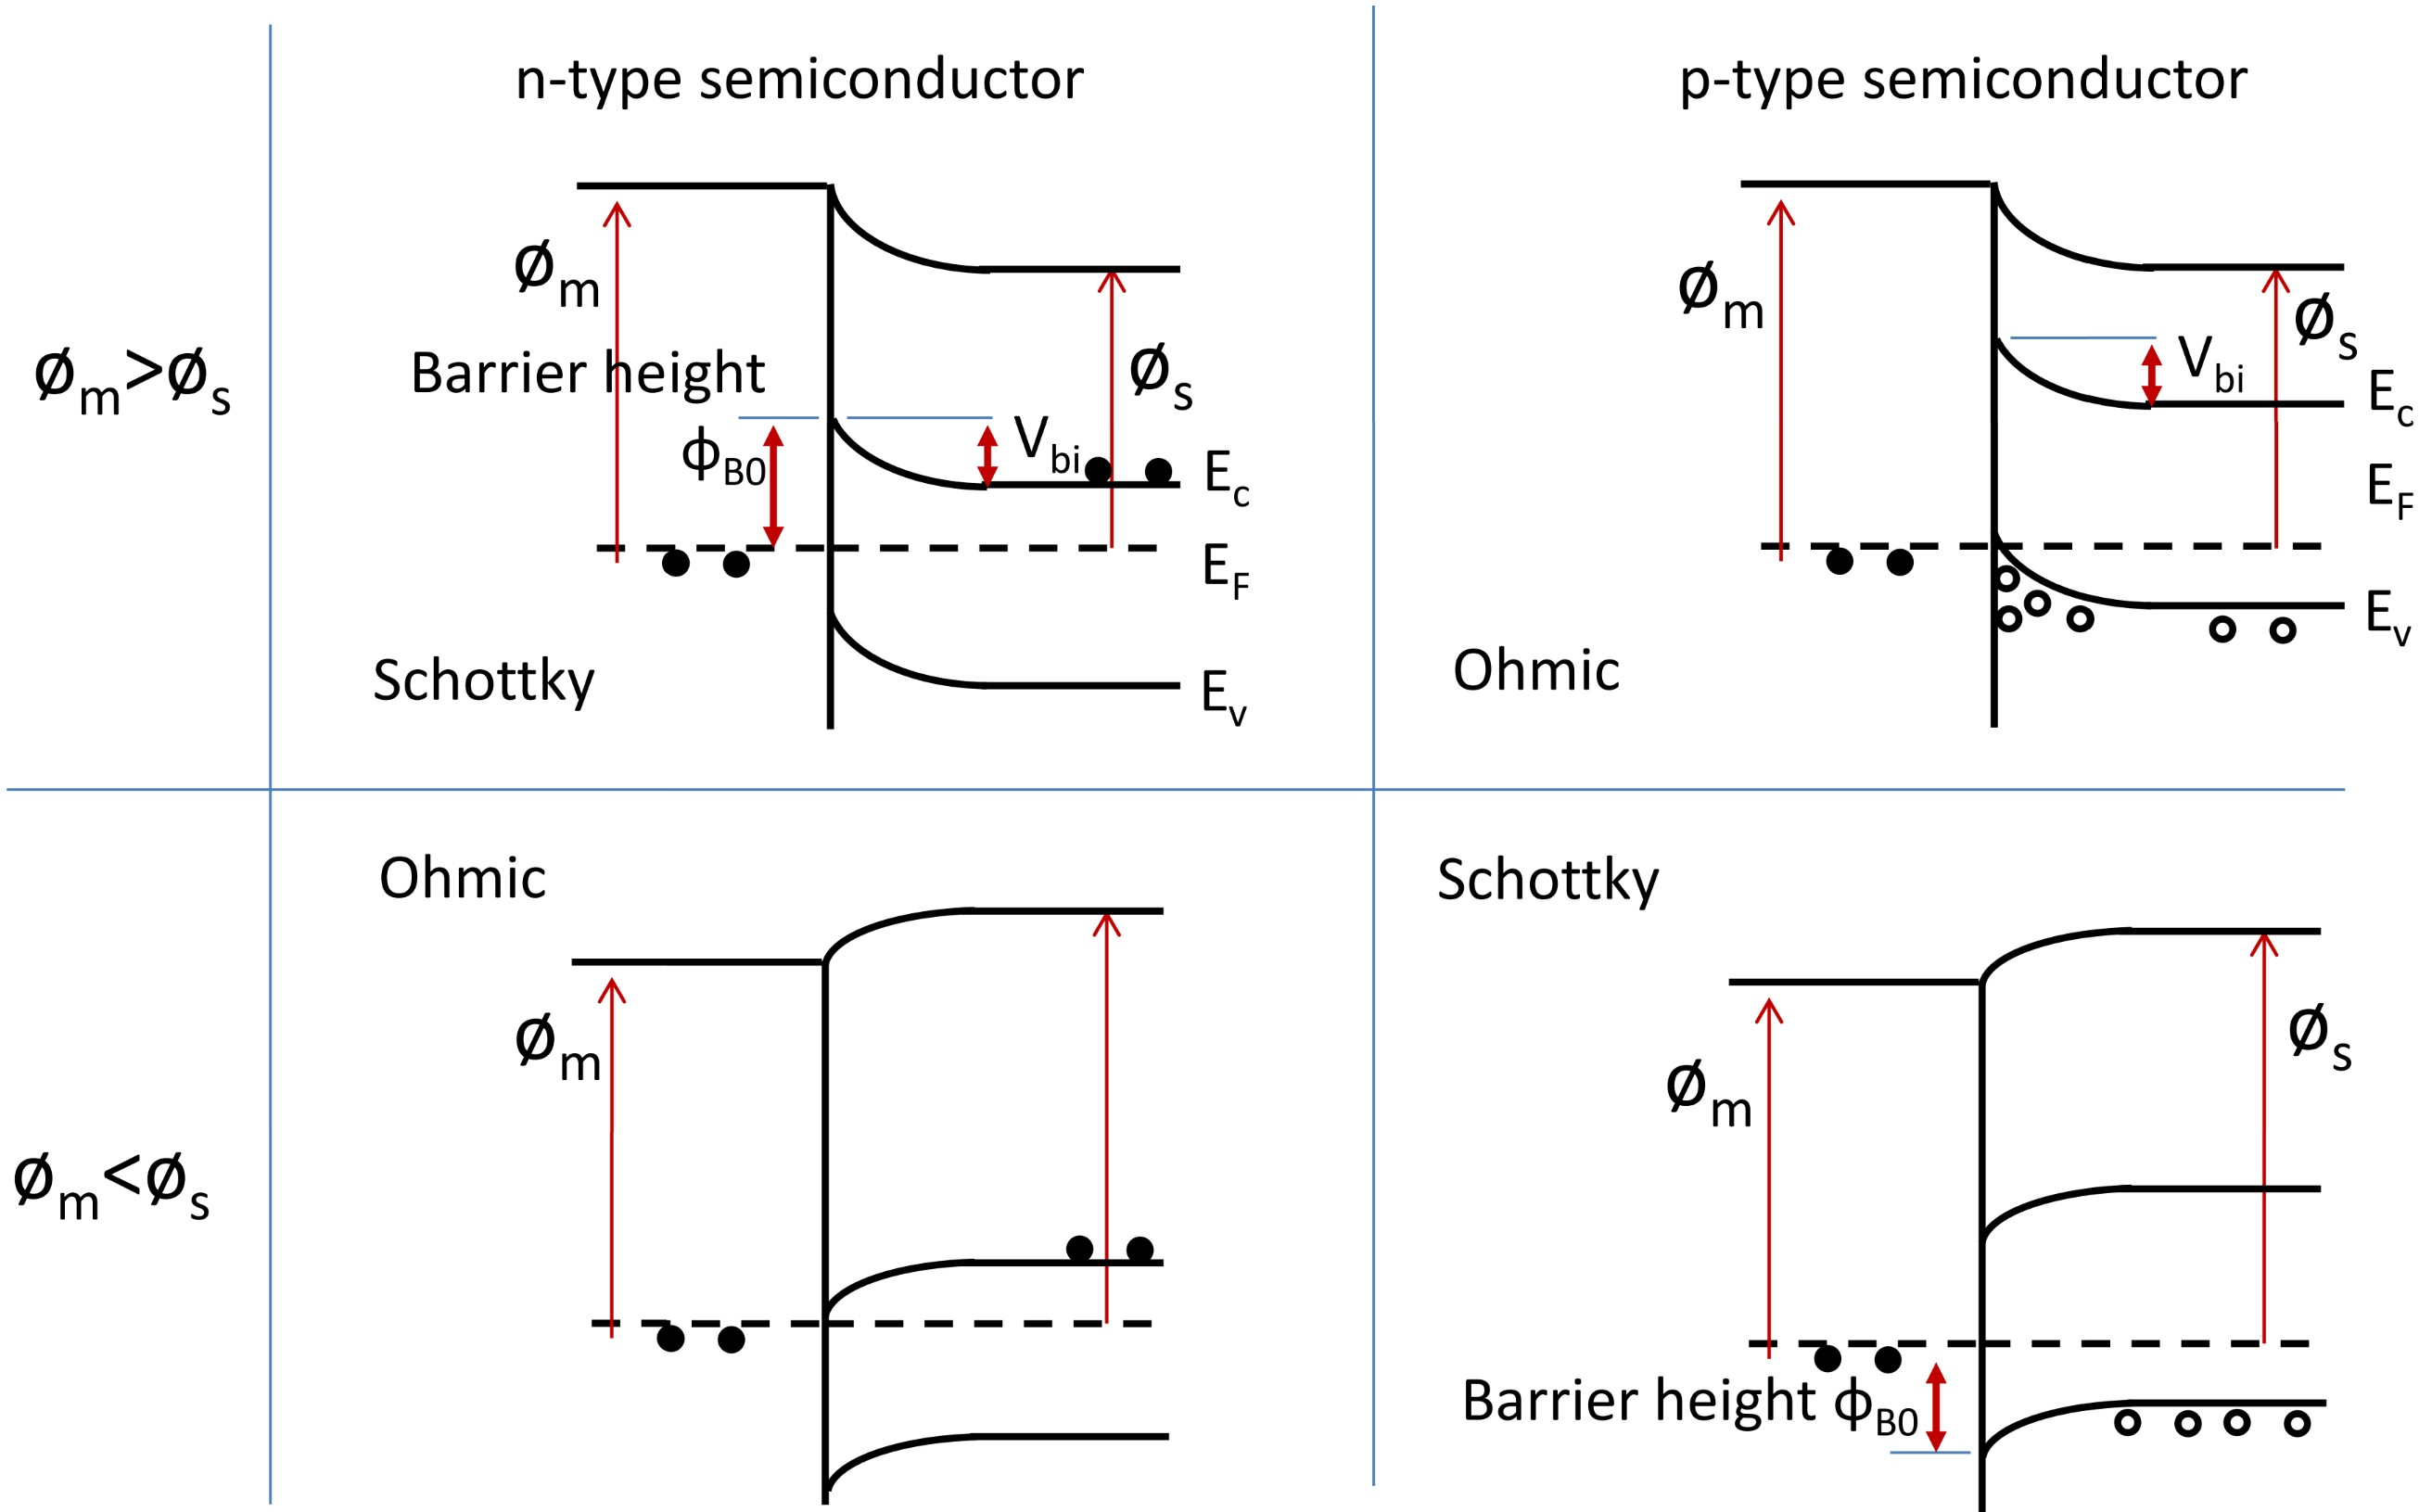
\includegraphics[width=\linewidth]{Types-of-semiconductor.jpg}
            \label{fig:Types-of-semiconductor.jpg}
        \end{figure}
    \end{frame}

    \begin{frame} \frametitle{Tunneling Barrier}
        \begin{figure}[H]
            \centering
            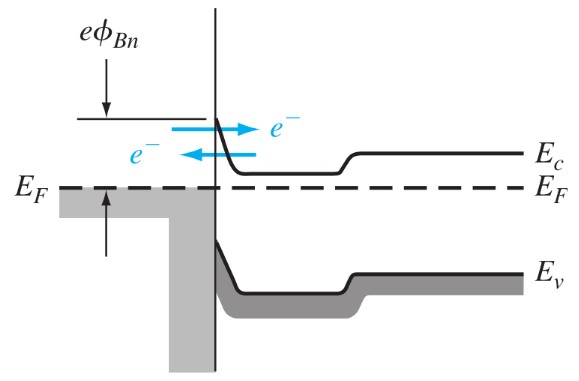
\includegraphics[width=0.6\linewidth]{Tunneling-barrier.jpg}
            \label{fig:Tunneling-barrier.jpg}
        \end{figure}
        \begin{equation*}
            \begin{aligned}
                J_t & \propto \exp \left( \frac{-e \phi_{Bn} }{E_{oo} }  \right) \\
                E_{oo} &= \frac{e \hbar}{2} \sqrt{\frac{N_d}{\varepsilon_s M_n^*} } 
            \end{aligned}
        \end{equation*}
    \end{frame}

    \begin{frame} \frametitle{Specific Contact Resistance}
        \par $R_c$ defined as the reciprocal of the derivative of current density with respect to voltage evaluated at zero bias.
        \begin{equation*}
            \begin{aligned}
                R_c &= \left. \left( \frac{\partial J}{\partial V}  \right)^{-1} \right|_{V = 0} \quad \Omega-cm^{2}  \\
                J_n &= A^* T^2 \exp \left( \frac{-e \phi_{Bn}}{kT}  \right) \left[ \exp \left( \frac{eV}{kT}  \right) - 1 \right] \\
                R_c &= \frac{\left(\frac{kT}{e} \right) \exp \left( \frac{+e \phi_{Bn} }{kT}  \right)}{A^* T^2} 
            \end{aligned}
        \end{equation*}
    \end{frame}

    \begin{frame} 
        \begin{center}
            \Large\textcolor{blue}{Good luck to your midterm exam!}
        \end{center}
    \end{frame}
\end{document} 